\documentclass[12pt,letterpaper]{report}
\usepackage[utf8]{inputenc}
\usepackage[T1]{fontenc}
\usepackage[english]{babel}
\usepackage{amsmath}
\usepackage{amsfonts}
\usepackage{amssymb}
\usepackage{graphicx}

\title{Charge Pump Derivation}
\author{Ryan J. Billing}

\begin{document}
	\maketitle
	\begin{figure}
		\centering
		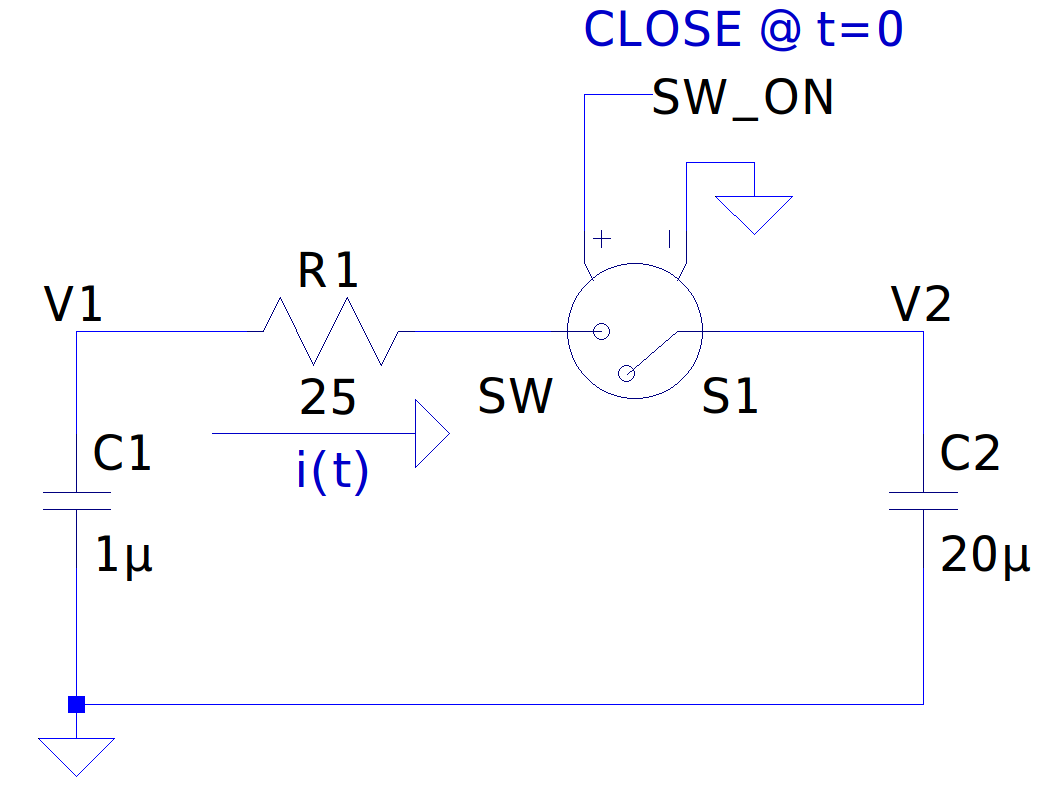
\includegraphics[width=0.7\linewidth]{img/charge_pump_discharge_cycle}
		\caption{Charge Pump discharge cycle operation}
		\label{fig:chargepumpdischargecycle}
	\end{figure}
	
	\section{Initial observations}
	Figure \ref{fig:chargepumpdischargecycle} depicts part of a charge pump circuit during the discharging cycle.  $C_1$ is the flying capacitor that was charged to a voltage of $V_1$.  At time $t=0$ the switch $S_1$ will close and $C_1$ will begin to discharge into $C_2$.
	
	The goal of this exercise is to determine how much energy is dissipated in R1 and determine the final voltage after the circuit has stabilized.  A closed-form solution for $i(t)$ is determined, it can be used to quantify how much charge is transferred from $C_1$ to $C_2$ in this scenario.   The final voltages, $V_1$ and $V_2$, can be determined from the integral of $i(t)$ by subtracting this charge from $C_1$ or adding it to $C_2$.  In the final settled state it is apparent that $V_1 = V_2$.
	
	\section{Useful relationships}
	This section presents a set of fundamental relationships that may be used to determine the function for $i(t)$.
	
	\begin{align}
		i(t) &= -C_1 \frac{dV_1}{dt} \label{c1deriv} \\
		i(t) &= C_2 \frac{dV_2}{dt} \label{c2deriv} \\
		i(t) &= \frac{V_1(t) - V_2(t)}{R_1} \label{itV}
	\end{align}

	\section{Derivation of i(t)}
	First find $V_1$ and $V_2$ from equations (\ref{c1deriv}) and (\ref{c2deriv}).  
	
	\begin{align}
		V_1(t) &= -\frac{1}{C_1} \int i(t) dt \text{ (Negative sign because current is going out of $C_1$)} \nonumber \\
		V_2(t) &= \frac{1}{C_2} \int i(t) dt
	\end{align}
	
	Plug these into (\ref{itV}) and then solve the resulting differential equation for $i(t)$.
	
	\begin{align}
		i(t) &= -\frac{1}{R_1} \bigg( \frac{1}{C_1} \int i(t) dt -\frac{1}{C_2} \int i(t) dt\bigg)
	\end{align}

	Next differentiate and collect like terms.
	
	\begin{align}
		\frac{di(t)}{dt} &= - \frac{\frac{1}{C_1} + \frac{1}{C_2}}{R_1} i(t) \nonumber \\
		R_1 \frac{C_1 C_2}{C_1 + C_2} \bigg ( \frac{1}{i(t)}\bigg) \frac{di(t)}{dt} &= -1
	\end{align}

	Integrating both sides.
	
	\begin{align}
		R_1 \frac{C_1 C_2}{C_1 + C_2} \int \frac{1}{i(t)} dt  &= \int -1 dt \\
		R_1 \frac{C_1 C_2}{C_1 + C_2} \bigg( ln\big(i(t)\big) + C\bigg) &= -t \\
		ln\big(i(t)\big) + C &= -t  \frac{C_1 + C_2}{R_1 C_1 C_2}
	\end{align}

	Exponentiate to solve for $i(t)$,
	
	\begin{align}
		e^{ln\big(i(t)\big)} e^{C} &= e^{-t \frac{C_1 + C_2}{ R_1C_1 C_2}} \nonumber \\
		i(t) &= e^{-C} e^{-t  \frac{C_1 + C_2}{ R_1C_1 C_2}} \label{it_general}
	\end{align}

	Finally the integration constant can be determined by considering the initial conditions,
	
	\begin{align}
		i(0) &= \frac{V_1(0) - V_2(0)}{R_1}
	\end{align}

	The expression (\ref{it_general}) is solved for the known initial conditions at $t=0$ to determine the yet unknown constant of integration.  In this case the constant $C$ itself is a "don't care" quantity as we really want to know $e^{-C}$ directly.
	
	\begin{align}
		\frac{V_1(0) - V_2(0)}{R_1} &=  e^{-C} e^{-0  \frac{C_1 + C_2}{R_1 C_1 C_2}} \nonumber \\
		 \frac{V_1(0) - V_2(0)}{R_1} &=  e^{-C} 1 \nonumber \\
		 e^{-C} &= \frac{V_1(0) - V_2(0)}{R_1} \label{intconst}
	\end{align}

	Plugging (\ref{intconst}) into(\ref{it_general}), a closed-form expression for the resistor current, $i(t)$, is obtained.
	
	\begin{align}
		i(t) &= \frac{V_1(0) - V_2(0)}{R_1}  e^{-t \frac{(C_1 + C_2)}{R_1 C_1 C_2}} 
	\end{align}
	
	Then to help tidy the appearance of things, let
	
	\begin{align}
		V_{i1} &= V_1(0)   \\
		V_{i2}  &=  V_2(0) \\
		\tau &= \frac{1}{ \frac{C_1 + C_2}{R_1 C_1 C_2} } = R_1 \frac{C_1 C_2}{C_1 + C_2}
	\end{align}

	And then the final expression reveals a familiar time domain response. In fact, the circuit could be redrawn as a single capacitor and resistor network driven by a step response with amplitude $V_{i1} - V_{i2}$, and where the capacitor value is equivalent to the series combination of $C_1$ and $C_2$.
	
	\begin{align}
	i(t) &= \frac{V_{i1} - V_{i2}}{R_1}  e^{-\frac{t}{\tau}} 
	\end{align}

	\section{Determine final settled voltage}
	Either one of two approaches may be used to determine the final voltage measured at nodes $V_1 = V_2$.  One approach integrates the current, $i(t)$, to determine the charge transferred and then using the formula $Q=CV$ to solve for the final voltage.  
	
	A second approach looks directly to energy lost during the stabilization, or,
	\begin{align}
		E_{R1} = R_1 \int_{0}^{\infty} i(t)^2 dt
	\end{align}

	\subsection{Charge based approach}
	The total charge transfer is the following.
	\begin{align}
	Q_{R1} &= \frac{V_{i1} - V_{i2}}{R_1}  \int_{0}^{\infty}  e^{-\frac{t}{\tau}} dt \nonumber \\
	&= \frac{V_{i1} - V_{i2}}{R_1}   \bigg[ -\tau e^{-\frac{t}{\tau}} \bigg ]_{0}^{\infty} \nonumber \\
	&= \frac{V_{i1} - V_{i2}}{R_1}  \bigg[ 0 - \big ( -\tau e^{-\frac{0}{\tau}} \big) \bigg ] \nonumber \\
	&= \tau \frac{V_{i1} - V_{i2}}{R_1}
	\end{align}	

	Next it is observed that the same amount of charge leaves $C_1$ and is added to $C_2$.  The final charge, $Q_f$, can be expressed in terms of either $V_1$ or $V_2$ as follows.
	
	\begin{align}
	Q_{f1} &= C_1 V_{i1} - Q_{R1} = C_1 V_f \nonumber \\
	Q_{f2} &= C_2 V_{i2} + Q_{R1} = C_2 V_f
	\end{align}

	Picking one,
	\begin{align}
		Q_{f2} &= C_2 V_{i2} + \tau \frac{V_{i1} - V_{i2}}{R_1} \label{qfv2}
	\end{align}

	Since the quantity $V_f$ is wanted, the expression (\ref{qfv2}) is solved.
	\begin{align}
		C_2 V_f &= C_2 V_{i2} + \tau \frac{V_{i1} - V_{i2}}{R_1}  \nonumber \\
		V_f &= V_{i2} + \tau \frac{V_{i1} - V_{i2}}{R_1 C_2} \label{vfinal_cg_based}		
	\end{align}

	\subsection{Energy based approach}
	Combined with knowledge of energy stored in capacitors,
	\begin{align}
		E_{FINAL} &= E_{C1} + E_{C2} - E_{R1} \nonumber \\
		&= \frac{1}{2} (C_1+C_2)V_{FINAL}^2 \label{efinal}
	\end{align}
	where,
	\begin{align}
		E_{C1} &= \frac{1}{2}C_1V_1^2 \nonumber\\
		E_{C2} &= \frac{1}{2}C_2V_2^2
	\end{align}

	And then the expression for $E_{R1}$ is determined by the following,
	\begin{align}
		E_{R1} &= R_1 \int_{0}^{\infty} \bigg( \frac{V_{i1} - V_{i2}}{R_1}  e^{-\frac{t}{\tau}}  \bigg)^2 dt \nonumber \\
		&=R_1 \bigg( \frac{V_{i1} - V_{i2}}{R_1}  \bigg)^2 \int_{0}^{\infty}    e^{-\frac{2t}{\tau}}  dt \nonumber \\
		&=  \frac{\big(V_{i1} - V_{i2}\big)^2}{R_1}  \bigg[ \frac{\tau}{2} e^{-\frac{2t}{\tau}} \bigg]_{0}^{\infty} \nonumber\\
		&=  \frac{\big(V_{i1} - V_{i2}\big)^2}{R_1}  \bigg[ \frac{\tau}{2} e^{-\frac{2(0)}{\tau}} - \frac{\tau}{2} e^{-\frac{2(\infty)}{\tau}} \bigg] \nonumber \\
		&=  \frac{\big(V_{i1} - V_{i2}\big)^2}{R_1}  \bigg[ \frac{\tau}{2}  - 0 \bigg] \nonumber \\
		&= \frac{\tau}{2R_1} \big(V_{i1} - V_{i2}\big)^2
	\end{align}
	
	Then (\ref{efinal}) is expanded.
	\begin{align}
		\frac{1}{2} (C_1+C_2)V_{FINAL}^2 &= \frac{1}{2}C_1V_{i1}^2 +\frac{1}{2}C_2V_{i2}^2 - \frac{\tau}{2R_1} \big(V_{i1} - V_{i2}\big)^2 \nonumber \\
		V_{FINAL}^2 &= \frac{C_1V_{i1}^2 +C_2V_{i2}^2 - \frac{\tau}{R_1} \big(V_{i1} - V_{i2}\big)^2}{C_1+C_2} \nonumber \\
		V_{FINAL} &= \sqrt{\frac{C_1V_{i1}^2 +C_2V_{i2}^2 - \frac{\tau}{R_1} \big(V_{i1} - V_{i2}\big)^2}{C_1+C_2}} \label{vf_energy_based}
	\end{align}
	
	With sufficient substitution and algebraic manipulation of (\ref{vf_energy_based}) the expression stated in (\ref{vfinal_cg_based}) can be obtained even though equivalence is not immediately apparent.  The expression for final voltage from the energy-based approach shows how the charge-based approach is less work.

\end{document}